\section{Using SEISCONF to modify parameter files}

By \textbf{Bladimir Moreno}

\textbf{Introduction}

The SEISCONF program is a JAVA application for editing some of the configuration files defined in the SEISAN earthquake analysis software. The editing is based on a simple Graphical User Interfaces composed of dialog-boxes where the input data is validated and an on-line help about the parameter being configured is given. The user-friendly interface allows to minimize the possible error in the configuration file format as well as to avoid unrealistic values for a particular parameter. SEISCONF was developed with Visual Cafe 4 standard edition. The software operates on Unix and Windows. 

When all settings are done as described under Installation, you can start the program from the prompt line as with the command `seisconf'. 

\textbf{Program options}

The program starts with a main window (Fig. \ref{fig:main-window}) with three options: 
(1) Edit the general SEISAN configuration parameters 
(\texttt{SEISAN.DEF}), (2) Edit the parameters for the hypocenter 
determination (\texttt{STATION?.HYP}) and (3) Edit the parameters for the 
waveforms analysis tool (\texttt{MULPLT.DEF}). An option can be selected 
by clicking the associated button. Normally these files are expected 
to be in the DAT directory. If the selected configuration file is 
found in the current directory, the user is prompted for choosing 
which file, either the local or the global. 

%\textbf{test png}
%
%\begin{figure}
%\htmlimage{scale=1.0}
%\centerline{
\includegraphics[width=0.9\linewidth]{fig/jens}}
%\caption{png.}
%\end{figure}

\begin{figure}
\htmlimage{scale=2.0}
\centerline{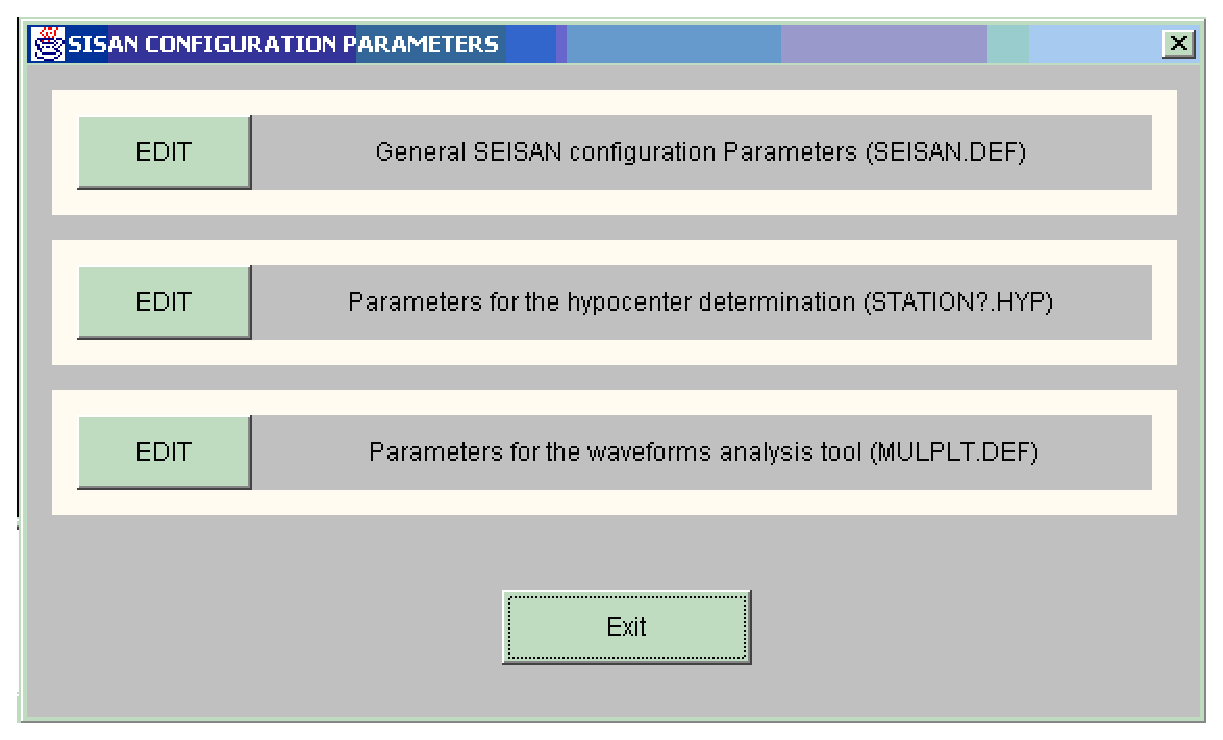
\includegraphics[width=0.9\linewidth]{fig/fig2}}
%\centerline{\includegraphics[width=0.9\linewidth]{fig/fig2.ps}}
\caption{Main Window of the program.}
\label{fig:main-window}
\end{figure}

\textbf{Changing SEISAN.DEF}

The editing process is based on a list made up with the configuration 
parameters. The parameters which are present in the configuration 
file are marked with ``*'' (Figure \ref{fig:main-window}). Parameters 
that are not found in the file, are set to defaults values. These 
default values are taken from the file \texttt{SEISANDEF.INP}. The user 
navigates through the list and can edit the associated values by using 
the edit-boxes labelled as VALUE1 and VALUE2. The entered data is 
validated according to the type and allowed range of values. The check-box 
labelled as ``Use'' permits to select/unselect the selected parameter 
to be saved in the configuration file. The button $<$Add New$> $ allows 
add a new parameter, same type of the one selected in the list, if 
possible. A brief description about the meaning of the selected parameter 
is given at the bottom of the window. 

\begin{figure}
\htmlimage{scale=2.0}
\centerline{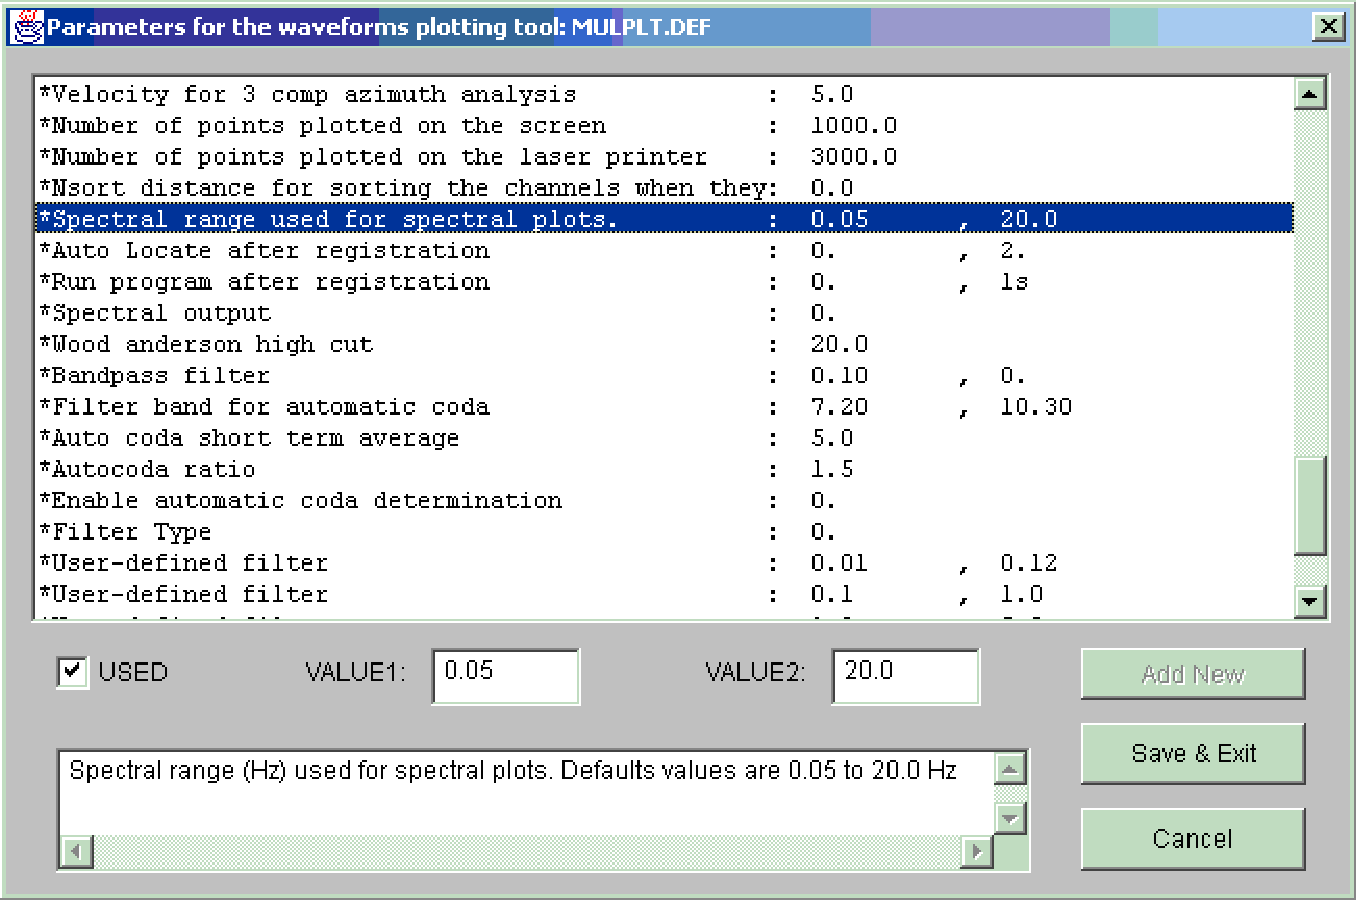
\includegraphics[width=0.9\linewidth]{fig/fig3}}
\caption{Edit Window of the configuration file: \texttt{MULPLT.DEF}}
\label{fig:edit-mulplt.def}
\end{figure}

\textbf{Changing STATION?.HYP}

The editing window (Figure \ref{fig:edit-mulplt.def}) is composed of 
four blocks: (1) A list with the general parameters (RESET TEST) of 
the HYPOCENTER program, (2) The seismic stations list, (3) The velocity 
model and (4) The control line. In addition there is a edit-box for 
the reporting agency and a combo-box labelled as \"Model\" for selecting 
which \texttt{STATION?.HYP} file is being edited. The question mark (?) in the 
file name takes the value selected in the combo-box. By default, 
\texttt{STATION0.HYP} is selected. The combo-box is made up from the set of 
station files (\texttt{STATION?.HYP}) found in the DAT directory or in the 
current local directory. There is two buttons $<$add$>$ and $<$remove$>$ 
in the station list block and velocity model block. Their function 
is for adding or removing items from the list. If you want to add 
a new item and there is one already selected (highlighted), you must 
click the button $<$add$>$ and then change the value with the new one. 
Do not try to enter the data before clicking the button $<$add$>$ 
because that will modify the current value of the selected item. The 
editing process is similar as it was explained in the previous section, 
except that the data for validation and on-line help is taken from 
the file \texttt{STATIONDEF.INP}. 


\begin{figure}
\htmlimage{scale=2.0}
\centerline{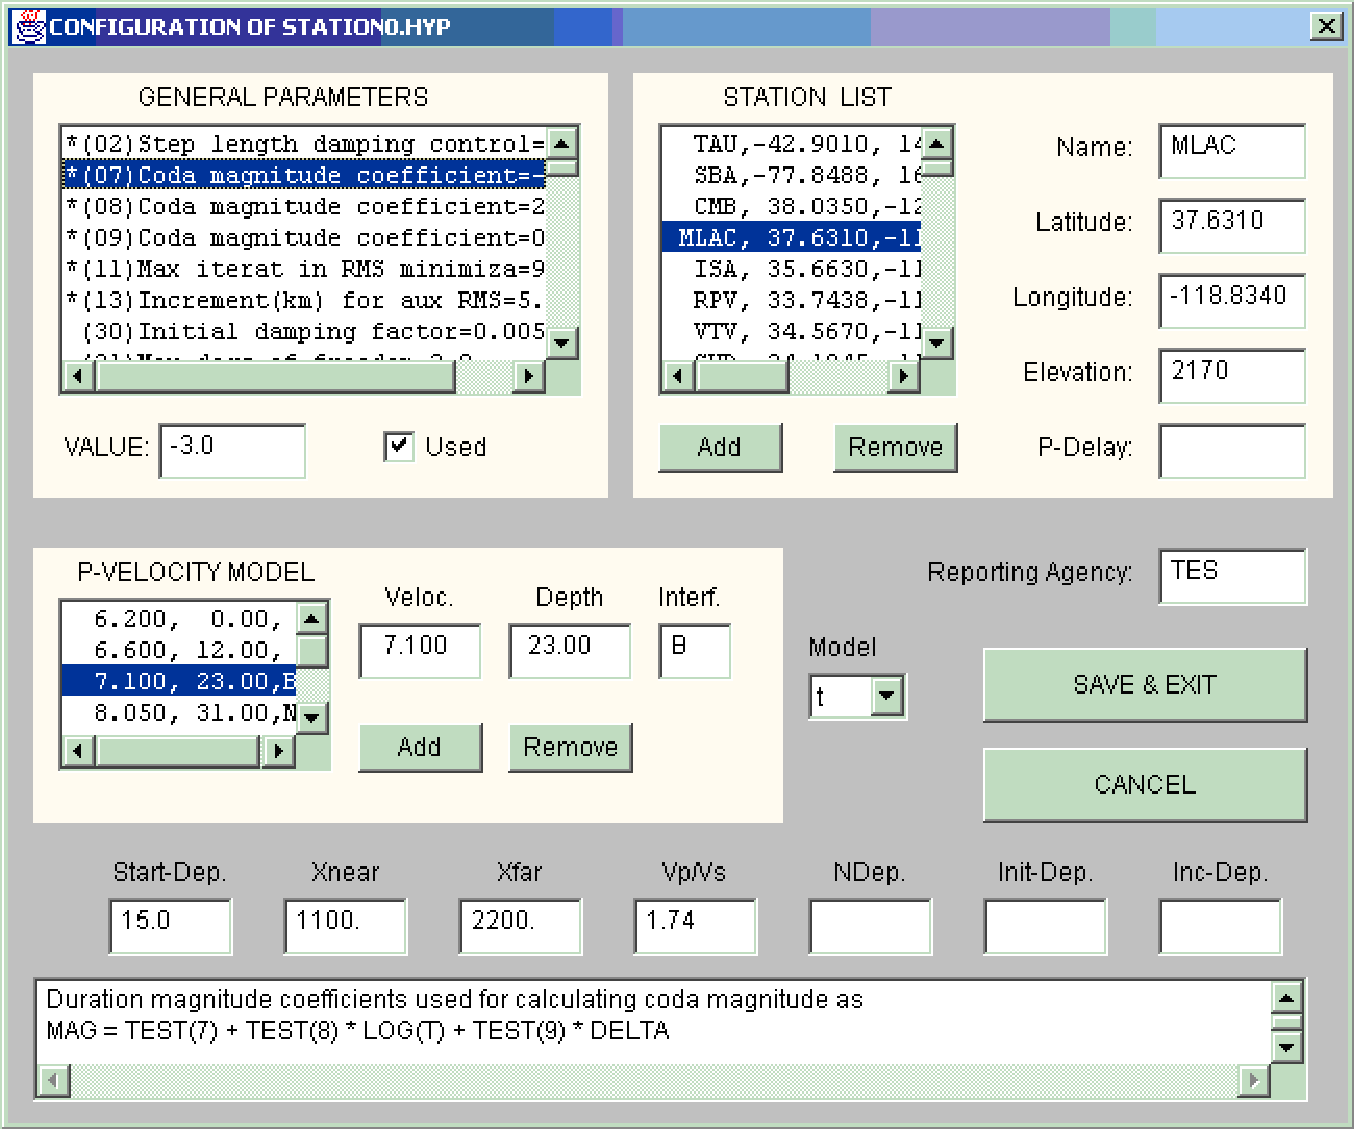
\includegraphics[width=0.9\linewidth]{fig/fig4}}
\caption{Edit Window of the configuration file: \texttt{STATION0.HYP}}
%\label{fig:}
\end{figure}

\textbf{Changing \texttt{MULPLT.DEF}}

The changing is the similar to \texttt{SEISAN.DEF}. The data for validation 
and on-line help is taken from \texttt{MULPLTDEF.INP}. 

\textbf{Input definition file format}

The input files \texttt{SEISANDEF.INP}, \texttt{MULPLTDEF.INP} and 
\texttt{STATIONDEF.INP} are used for data validation purpose and 
user's help support. Normally the user will not edit these files. The first two lines of the files are comments followed by three or more lines for each parameter: (1) The data numerical description, (2) The name and a short description of the parameter shown on the list and 
(3) A longer description (help) about the meaning of the parameter(s). This can be several lines. The data numerical description has the following format: 

$<$Keyword$>$:$<$default$>$,$<$range$>$,$<$value1$>$,$<$value2$>$,...;$<$type$>$,$<$column$>$,$<$width$>$,$<$dec$>$|... 

$<$keyword$>$: Identify the name of the parameter used in the configuration file.\newline
$<$default$>$: Default value used when the parameter is not found in the configuration file.\newline
$<$range$>$: A character for specifying when the parameter is enclosed by a range of values or is allowed to take a set of values. It is set with `R' for range or `U' for a set (see example below). \newline
$<$value1$>$,$<$value2$>$: Represent the lower and upper limit of the range of values which are allow to be 
taken. It is make sense when `R' is used in the $<$range$>$ option. When using `U', then newline
$<$value1$>$,$<$value2$>$,..,$<$valueN$>$ are the set of permitted values. \newline
$<$type$>$: A character for identifying the type of data: `F' float,`I' integer,`S' string of characters. \newline
$<$column$>$: The position (column) of the parameter in the configuration file. \newline
$<$width$>$: The number of characters occupied in the configuration file. \newline
$<$dec$>$: The number of digits after the point for float values. 

When more than one value is taken for a particular parameter, then the character `$|$' is used for 
dividing the two formats. 

Examples: 

SPECTRAL F-BAND:0.05,R,0,20 ; F,40,5,2 | 20.0,R,0,20 ; F,50,5,2 

The keyword \"SPECTRL F-BAND\" has two values. The first one is set by default to 0.05 Hz and can take values between 0 and 20 Hz. It is a float value found in the column 40 of the configuration file and occupies 5 characters with 2 decimal digits. The second value is set by default to 20 Hz and has the same numerical format as the first one, except that it is found in  column 50 of the configuration file. 

MAP\_SERVER:0,U,0,1,2,3,4,5 ; I,40,1 

The keyword \"MAP\_SERVER\" is set by default to 0 and can only take the values 0,1,2,3,4 and 5. It is 
an integer data found in column 40 and occupies a 1 character position. 

WAVEFORM\_BASE:BER ; S,40,5 

The keyword \"WAVEFORM\_BASE\" is set by default to \"BER\". It is a string with a maximum of 5 characters and it is found in the column 40 of the configuration file. 

Below is shown part of the content of \texttt{MULPLTDEF.INP} 

\verbatiminput{include/MULPLTDEF.INP}



